%% Template for EU deliverable, using the deliverable.sty style file

\documentclass[12pt,a4paper,twoside]{article}

%% common package
\usepackage[headers]{deliverable}
\usepackage{xspace}
\usepackage{verbatim}
\usepackage[usenames]{color}
\usepackage{listings}
\usepackage[usenames,dvipsnames,table]{xcolor}
\usepackage[pdftex,dvips]{graphicx}
\usepackage{url}
\usepackage{array}
%%

%%insert here other packages needed by sections

%%

%%%%%%%%%%%%%%%%%%%%%%%%%%%%%%%%%%%%%%%%%%%%%%%%%%%%%%%%%%%%%%%%%%%%%%%%%%%%%%
%%% Titlepage
%%%%%%%%%%%%%%%%%%%%%%%%%%%%%%%%%%%%%%%%%%%%%%%%%%%%%%%%%%%%%%%%%%%%%%%%%%%%%%

% declaration of variables used in style
\deliverableDocnumber{D3.2}
\deliverableTitle{Local solver in compliant-world cases}

\deliverableAuthor{Vincent Padois$^{1,2}$}
\deliverableResponsiblePartner{UPMC}
\deliverableAffiliation{% Insert here authors affiliations
 $^1$ Sorbonne Universit\'es, UPMC Paris 06, UMR 7222, Institut des Syst\`emes Intelligents et de Robotique (ISIR), F-75005, Paris, France.
 
 $^2$ CNRS, UMR 7222, Institut des Syst\`emes Intelligents et de Robotique (ISIR), F-75005, Paris, France.
}


\deliverableCoordinator{Vincent Padois}
\deliverableActivityNumber{n} %% n=1,..,10
\deliverableActivity{Local solver in compliant-world cases}
\deliverableDoctype{Deliverable} %% or Prototype
\deliverableClassification{Public} % or Consortium
\deliverableDistribution{Consortium} %
\deliverableStatus{Final} % Draft or Final
\deliverableDeliveryDate{28/2/2016}
\deliverableFile{D3.2.pdf} % please do not use "-" in the name
\deliverableVersion{1.0}
\deliverableDate{Feb.~28, 2016}
\deliverableYear{2016}
\deliverablePages{\pageref{LastPage}}
\deliverableChangelog{}
\deliverableProjectStartingDate{1st March 2013}
\deliverableProjectEndDate{28th February 2017}
\deliverableProjectAcronym{CoDyCo}
\deliverableProjectTitle{Whole-Body Compliant Dynamical Contacts in Cognitive Humanoids}
\deliverableContractNumber{600716}
\deliverableProjectCoordinator{Istituto Italiano di Tecnologia}
\deliverableProjectUrl{www.codyco.eu}
\deliverableFrameworkProgramme{FP7}
 
\deliverableWorkpackage{WP3}
\deliverableEditors{Vincent Padois}
\deliverableContributors{Morteza Azzad, Mingxing Liu, Mike Mistry, Francesco Nori, Vincent Padois, Daniele Pucci, Francesco Romano, Silvio Traversaro}

\deliverableAbstract{This deliverable provides an overview of the whole-body control strategies proposed within the framework of the CoDyCo project for balancing by means of compliant contacts. We first recall the general structure of the whole-body controller used in the CoDyCo project. This controller is written as a quadratic multi-objective optimization problem under linear constraints and priorities between the objectives can be dealt with through strict of soft hierarchy. This controller has to be modified in order to deal with compliant cases and two cases are then distinguished. In the first one, a contact model is supposed to be known and using that knowledge a control strategy is derived. In the second case, no model of the environment is assumed to be known and an adaptive force regulation task is added in order to account for the compliance of the environment. This deliverable is strongly related to deliverable 5.3 CITE{deliverable53} which discusses the technical details and choices for the implementation of the year-3 validation scenario.}
\deliverableReviewers{}
\deliverableKeywordList{Whole-body controllers, Non-rigid contacts, Multi-contacts, Goal-oriented tasks.}

%%%%%%%%%%%%%%%%%%%%%%%%%%%%%%%%%%%%%%%%%%%%%%%%%%%%%%%%%%%%%%%%%%%%%%%%%%%%%%
%%% Sections
%%%%%%%%%%%%%%%%%%%%%%%%%%%%%%%%%%%%%%%%%%%%%%%%%%%%%%%%%%%%%%%%%%%%%%%%%%%%%%

%% constants
\newcommand{\botegoCaps}{BOTEGO}
\newcommand{\certhCaps}{CERTH}
\newcommand{\cybionCaps}{CYBION}
\newcommand{\nuigCaps}{NUIG}
\newcommand{\ubitechCaps}{UBITECH}
%%

%%%%%%%%%%%%%%%%%%%%%%%%%%%%%%%%%%%%%%%%%%%%%%%%%%%%%%%%%%%%%%%%%%%%%%%%%%%%%%
%%% Misc. by Vincent
%%%%%%%%%%%%%%%%%%%%%%%%%%%%%%%%%%%%%%%%%%%%%%%%%%%%%%%%%%%%%%%%%%%%%%%%%%%%%%
\usepackage{titlesec}
\newcommand{\sectionbreak}{}
\graphicspath{{./figure/}}
\usepackage{pdfpages}
\usepackage{caption}
\usepackage{subcaption}
\usepackage{slashbox}
\usepackage{multirow}
\usepackage{appendix}
\usepackage{amsmath} % assumes amsmath package installed
\usepackage{amssymb}  % assumes amsmath package installed
\usepackage[ruled,vlined,linesnumbered]{algorithm2e}
\usepackage{mathtools}
\usepackage{graphicx}
\usepackage{hyperref}
\hypersetup{
    bookmarks=true,         % show bookmarks bar?
    unicode=false,          % non-Latin characters in Acrobat’s bookmarks
    pdftoolbar=true,        % show Acrobat’s toolbar?
    pdfmenubar=true,        % show Acrobat’s menu?
    pdffitwindow=false,     % window fit to page when opened
    pdfstartview={FitH},    % fits the width of the page to the window
    pdftitle={D11\_iCubSimulator.pdf},    % title
    pdfauthor={Vincent Padois},     % author
    pdfsubject={Local solver in rigid-world cases},   % subject of the document
    pdfcreator={Vincent Padois},   % creator of the document
    pdfproducer={Vincent Padois}, % producer of the document
    pdfkeywords= {}, % list of keywords
    pdfnewwindow=true,      % links in new window
    colorlinks=true,       % false: boxed links; true: colored links
    linkcolor=black,          % color of internal links (change box color with linkbordercolor)
    citecolor=black,        % color of links to bibliography
    filecolor=black,      % color of file links
    urlcolor=black           % color of external links
}

\newcommand{\vect}[1]{\mbox{\boldmath${#1}$}}%$
\newcommand{\av}{\vect{\chi}}
\newcommand{\tens}[1]{#1}
\DeclareMathOperator*{\argmin}{argmin}

%%%%%%%%%%%%%%%%%%%%%%%%%%%%%% BEGIN DOCUMENT
\begin{document}

\deliverableMaketitle

%%TODO move to style
\newcolumntype{L}[1]{>{\raggedright\let\newline\\\arraybackslash\hspace{0pt}}m{#1}}
\newcolumntype{C}[1]{>{\centering\let\newline\\\arraybackslash\hspace{0pt}}m{#1}}
\newcolumntype{R}[1]{>{\raggedleft\let\newline\\\arraybackslash\hspace{0pt}}m{#1}}

\textbf{Document Revision History}
\begin{center}
\begin{tabular}{|C{2cm}|C{3cm}|C{5cm}|C{4cm}|}
\hline
\textbf{Version}&\textbf{Date}&\textbf{Description}&\textbf{Author}\\\hline
v.~0.1 & Jan.~19, 2016 & Initial creation of the file & Vincent Padois\\ \hline
v.~0.9 & Feb.~25, 2016 & Final version & Vincent Padois \\ \hline
v.~1.0 & Feb.~28, 2016 & Proofread version & Francesco Nori \\ \hline
\end{tabular}
\end{center}
 
 \clearpage

\newpage
\renewcommand*\contentsname{Table of Contents}
\renewcommand*\listfigurename{Index of Figures}
\tableofcontents
\newpage
\listoffigures
\newpage

%%%%%%%%%%%%%%%%%%%%%%%% Start deliverable content here.

\section{Introduction}


Under-actuated robots, such as free-floating humanoid robots, usually need to make contacts with their environments to achieve some goal directed whole-body movements. Most researches on whole-body control assume that the environment of the robot is rigid. This means that no adaptation to the environment compliance is needed for controllers. In reality, there is no completely rigid surface even if in practice we can assume a surface to be rigid if it is stiff enough (i.e. deflection is negligible). Unfortunately, many objects in human environments cannot be considered as stiff enough and their compliance has to be accounted for (e.g. a soft cushion, a sofa, a yoga carpet). Indeed, a controller that does not take into account the compliant  properties of the contact material may not be sufficient:  the compliance of
the contact has to be considered by the controller, otherwise the robot may fail to properly balance and fall over. For example, %pushing too strongly against a rigid object may result in damages to the robot or the environment; and 
pushing too weakly against a compliant object may not provide the robot with enough reaction forces to support its whole-body tasks. The problem is complex as the rigidity of the object in contact is unknown a priori to robotic controllers, which is usually the case in many scenarios.\\
 

The humanoid whole-body control problem has been addressed by different types of whole-body controllers, using analytical approaches \cite{Khatib08,Sentis10,Righetti13}, constrained quadratic programming \cite{Abe07,Liu11,Salini11,Salini13,Saab13}, or a mixture of them \cite{Stephens10,Nori15}. These controllers are either developed for rigid environments, or validated only in rigid contact scenarios.
In general, a valid set of contact forces during whole-body task control can be found by solving a multi-objective problem with a set of elementary task objectives as well as constraints, such as whole-body dynamics, friction cone constraints for non-sliding contacts, and linear complementarity conditions \cite{Muico09,Saab13,Salini11,Salini13}, which implies zero relative motions between two bodies in contact when normal contact force is non-negative. In the case of rigid contact with static environment, the linear complementarity condition implies two constraints: (i) the motion of the contact point is zero and (ii) the contact force along the normal to the contact surface is non-negative.  The zero motion constraint may not necessarily be true in the case of non-rigid contacts, since the velocities or accelerations of contact points may be non-zero, although the relative motion between the two contact points remains zero. In this case, hybrid control methods \cite{khatib87} that control forces and motions in orthogonal directions are not applicable. Therefore, the controller should take into account the dynamic relation between the contact point position and the contact force, rather than just control the contact force alone.\\ 

Such physical interaction dynamics is taken into account in impedance control \cite{Hogan85} with the idea of controlling the relation between the contact point motion and the reaction force. Traditional impedance control \cite{Hogan85,Love95,Tsumugiwa02} computes the target impedance of the robot according to the estimated impedance of the environment, which requires high quality measurement of interaction forces. In \cite{Buchli10, Yang11}, learning approaches are applied to optimize the robot impedance. Such approaches do not require interaction force sensing and can be adaptable to variable environment impedance. However, the application of such approaches in the context of humanoid balance control with non-rigid contacts is not suitable. First, these methods rely on trajectory-based learning and adaptation algorithms, whereas there is not necessarily a reference motion trajectory for each support contact in the whole-body balancing context considered here. Furthermore, they need to explore the entire state-action space if a globally optimal solution is to be found, which is impossible for high dimensional robots such as humanoids.\\

The problem of humanoid balance control with deformable contact support was addressed in \cite{Bouyarmane11b}, which proposed a posture planning approach assuming that the contact material properties are known. Compliant contacts between robots and their environments have been studied by some researchers in other areas such as grasping \cite{Xydes&Kao99} and animated characters \cite{Jain&Liu11}. However, there has not been much research efforts on balancing legged robots on compliant surfaces.\\

This deliverable provides an overview of the whole-body control strategies proposed within the framework of the CoDyCo project for balancing by means of compliant contacts. It is organized as follows. We first recall the general structure of the whole-body controller used in the CoDyCo project. This controller is written as a quadratic multi-objective optimization problem under linear constraints and priorities between the objectives can be dealt with through strict of soft hierarchy. This controller has to be modified in order to deal with compliant cases and two cases are then distinguished. In the first one, no model of the environment is assumed to be known and an adaptive force regulation task is added to the original ``rigid contact" controller in order to account for the compliance of the environment. In the second case, a contact model is supposed to be known and using that knowledge a control strategy is derived.

\section{General structure of the whole-body controller in the CoDyCo project}

Even though it is not often formulated as such, control of dynamical systems is an optimization problem. Within the framework of the CoDyCo project, the whole-body controller is written as a quadratic multi-objective optimization problem under linear constraints where priorities between the objectives can be dealt with through strict of soft hierarchy. Deliverable 3.1 CITE{deliverable31} exposes the reasons why it is preferable to express controllers in this way. The logic behind this choice can be briefly summarized in a very straightforward way:
\begin{enumerate}
\item the equation of motion and joint space to task spaces mappings can be written as equalities but they are not sufficient to describe the overall dynamics and physical behaviour of a robot.
\item Indeed, other intrinsic physical constraint have to be accounted for at the joint level as well as in Cartesian space. These constraints do not solely describe relationships between physical quantities but also limits which cannot (control input saturation) or should never be crossed in order to maintain the robot and its environment in proper working conditions.
\item Theses limits translate into inequalities.
\item Assuming a convex solution space, the optimal solution of the control problem lie at the boundary of the feasible (constraint compliant) solution space.
\item Finding the optimal solution thus boils down to finding the active constraint set, \textit{i.e.} on which boundary it lies.
\item Optimization problem solvers are designed to optimally choose this subset of constraints that should be considered when computing the optimal solution of the control problem.
\item The strong mathematical background in convex optimization is such that optimization based methods mostly outperform analytical methods attempting to heuristically activate constraints.
\end{enumerate}

\subsection{Formulation}
Based on this formulation choice, the reactive control problem aims at finding at each control instant the actuation torque minimizing $T(\mathbb{X})$, some tasks related function to minimize, given the equation of motion of the multi-body system as well as other equality and inequality constraints. This can be written
\begin{subequations}\label{eq:one task}
%\begin{eqnarray}
%\vect{\tau}^*_{t} =~\argmin \limits_{\mathbb{X}_{t}} & T(\mathbb{X}_{t}, t) \label{eq:cp obj}\\  
%\text{subject to} 
%  & \mathbf{M}(\vect{q}_{t}) \vect{\dot{\nu}}_{t}+\vect{n}(\vect{q}_{t},\vect{\nu}_{t}) = \mathbf{S}\vect{\tau}_{t}+\mathbf{J}_c(\vect{q}_{t})^\top \vect{F}_{c,{t}} \label{eq:cp dyn model}\\ 
%  & \mathbf{A}(t) \mathbb{X}_{t}   =  \vect{b}(t)  \label{eq:cp eq cons} \\
%  & \mathbf{G}(t) \mathbb{X}_{t} \leq \vect{h}(t)  \label{eq:cp ineq cons}
%\end{eqnarray}
\begin{eqnarray}
{\tau}^* =~\argmin \limits_{\mathbb{X}} & T(\mathbb{X}) \label{eq:cp obj}\\  
\text{subject to} 
  & {M}(q) {\dot{\nu}}+{C}({q},{\nu}){\nu} + G(q) = {B} {\tau} + \underbrace{\sum_{k = 1}^{n_c} {J}^\top_{\mathcal{C}_k}(q) f_k}_{J^\top(q) f} \label{eq:cp dyn model}\\ 
  & {A}(q,\nu) \mathbb{X}   =  {b}(q,\nu)  \label{eq:cp eq cons} \\
  & {D}(q,\nu) \mathbb{X} \leq {h}(q,\nu)  \label{eq:cp ineq cons}
\end{eqnarray}               
\end{subequations}
where:
\begin{itemize}
\item $\tau \in \mathbb{R}^n$ is the internal actuation torque with $n + 1$ the number of rigid bodies -- called links -- connected by $n$ actuated joints with one degree of freedom each.
\item ${q} \in \mathbb{R}^3 \times SO(3)\times \mathbb{R}^n$ is the generalized coordinates that parametrizes the configuration of the free-floating system. $q$ is a triplet composed of the origin and orientation of the base frame expressed in the inertial frame $\left(\prescript{\mathcal{I}}{}p_{\mathcal{B}},\prescript{\mathcal{I}}{}R_{\mathcal{B}}\right)$ and the $n$ joint angles $q_j$.
\item ${\nu} \in \mathbb{R}^{n+6}$ is the system velocity, a triplet concatenating the floating-base twist $\left (^\mathcal{I}\dot{ p}_{\mathcal{B}},^\mathcal{I}\omega_{\mathcal{B}}\right)$ and the joint velocities ${\dot{q}}_j$.
\item ${J}({q})= \left[{J}^\top _{\mathcal{C}_1}({q})~ \dots~ {J}^\top _{\mathcal{C}_k}({q}) \right]^\top$ is the contact Jacobian matrix for all $k$ contact points.
\item $f= \left[ {f}^\top_{1}~ \dots~ {f}^\top_{k}~ \right]^\top $ is the vector of external contact wrenches applied by the environment on the links.
\item $\mathbb{X} = \left(\dot{\nu}, \tau, f \right)$ gathers the dynamic variables of the multi-body system.
\item ${M} \in \mathbb{R}^{n+6 \times n+6}$ is the mass matrix.
\item ${C} \in \mathbb{R}^{n+6 \times n+6}$ is the Coriolis and centrifugal effects matrix.
\item ${G} \in \mathbb{R}^{n+6}$ is the gravity term.
\item $B = (0_{n\times 6} , 1_n)^\top$ is a selection matrix.
\item ${A}(q,\nu) \mathbb{X}   =  {b}(q,\nu)$ gathers kinematics constraints related to the velocity of the contact points.
\item ${D}(q,\nu) \mathbb{X} \leq {h}(q,\nu)$ gathers inequality constraints related to joint limits (position and velocity), control input saturation, contact forces (existence and friction limits) and potentially obstacle avoidance.
\end{itemize}

\subsection{Dealing with multiple objectives}

The control problem is often multi-objective and the tasks-related function $T(\mathbb(X))$ can actually be written
\begin{equation}\label{eq:multi task}
T(\mathbb{X}) = T\left(\lambda_1, T_1(\mathbb{X}), \lambda_2, T_2(\mathbb{X}), \dots, \lambda_{n_t},T_{n_t}(\mathbb{X})\right)
\end{equation}
where $T_i(\mathbb{X})$ is the $i$-th task among $n_t$ operational tasks to be achieved with $J_i(q)$ its associated task Jacobian and $\lambda_i$ its priority level. $T_i$ is generally of three types:
\begin{equation}
\begin{array}{ll}
\bullet~~\text{Operational space acceleration} & T_i={J_i}({q}){\dot{\nu}} + {\dot{J}_i}({q}_t,{\nu}){\nu} -{\ddot{x}}^{d} \\
\bullet~~\text{Joint space acceleration}       & T_i={\dot{\nu}}-{\dot{\nu}}^{d} \\
\bullet~~\text{Operational space force}        & T_i={f}_{\mathcal{C}_i}-{f}_{\mathcal{C}_i}^{d}
\end{array}
\end{equation}
where ${\ddot{x}}^{d}$, ${\dot{\nu}}^{d}$ and ${f}_{\mathcal{C}_i}^{d}$ are desired Cartesian space acceleration, configuration space acceleration and contact wrench respectively, the desired value itself being the outcome of some higher level control architecture (Proportional--Derivative--Integral regulators and/or Momentum regulators and/or Model Predicitve Controllers and/or Trajectory planners providing a feedfoward reference, \textit{etc}).\\

$T_i$ usually appears in $T$ under the form of a weighted, euclidean norm thus leading to a quadratic cost associated to each task. This quadratic form and the linearity of the constraints allows to resort to the convex optimization techniques, more particularly Linear Quadratic Programs. Then, depending of the type of retained prioritization scheme, the optimization problem \ref{eq:one task} can be solved:
\begin{enumerate}
\item at once using a single LQP and soft prioritization where $T$ is written as a weighted sum of quadratic costs and where $\lambda$s play the role of weights for each task, see \cite{Salini2011,bouyarmane2011using} for examples;
\item using a cascade of LQPs thus inducing strict prioritization between tasks (in that case $\lambda$s are used to defined a lexicographic order), see \cite{Saab13,herzog2014balancing,hierarchicalq} for examples;
\item using a representation able to convey both soft and strict prioritization, see \cite{liu-AutRob2015,liu-AutRobSI2015}.
\end{enumerate}

\subsection{Direct and two-stage whole-body control approaches}

In CoDyCo, these three types of prioritization scheme coexist and are used indifferently as they allow to produce very similar types of behaviours\footnote{A formal comparison of their intrinsic properties is out of the scope of this deliverable but would constitute a work of interest for the community}. A distinction has still to be made between two ways to approach the whole-body control problem.\\

The first, direct, approach does not separate the problem of computing the contact forces from the one of computing the joint torques. Given some task space desired acceleration (among which a center of mass one), the resolution of the control problem described by Equation~(\ref{eq:one task}) directly provides the optimal torques. The contact forces come as a by-product of the problem resolution. This approach has the very nice property of being able to account for the joint level constraints. Its drawback is that it hides some of the essence of the balance control problem and while it may be preferable to use such a solution for practical implementation, a two-stage solution may be preferred to ease the analysis of the system (for example in terms of its controllability).\\

The second, two-stage approach, uses contact forces as intermediate controls and first compute the desired contact forces given the desired acceleration of the center of mass. This can be done using the Newton-Euler equation for the floating-base system, written at the center of mass of the system. It can be written
\begin{equation}
\label{equ:NE equation}
\left( \begin{array}{c}
m \ddot{x}\\ 
\dot{H}_{\omega}
\end{array}\right) =
m g + \underbrace{\sum_k \left(\begin{array}{cc}
S(p_{\mathcal{C}_k} - x) & 1_{3} \\
1_{3} & 0_{3\times 3}
\end{array}\right)  f_k}_{X_{\mathcal{C}} f}
\end{equation}
where $m$ is the total mass of the system, $x \in \mathbb{R}^3$ is the position of the center of mass expressed in the inertial frame, $\dot{H}_{\omega}$ is the derivative of the angular momentum, $g$ is the acceleration induced by gravity expressed in the inertial frame, $p_{\mathcal{C}_k}$ is the $k$-contact point and $S(u) \in \mathbb{R}^{3\times 3}$ is the skew-symmetric matrix such that $S(u)v = u \times v$, where $\times$ denotes the cross product operator in $\mathbb{R}^3$.\\

Equation~(\ref{equ:NE equation}) plainly displays the relation between contact wrenches and the dynamics of the center of mass and $f$ can be computed based on it in order to achieve some desired center of mass linear acceleration $\ddot{x}^d$ and to maintain the angular momentum null (by choosing $\dot{H}_{\omega} = 0$). The solution for $f$ can be computed using an LQP as well. This allows to account for inequality constraints related to friction. Given these desired contact forces, the whole-body control problem can then be solved using the general formulation provided by Equation~(\ref{eq:one task}). This control approach, often referred as \textit{momentum-based balance controller}, has extensively been used in the recent years \cite{Lee&Goswami12,perrin_ISRR2015,Herzog2015} and is the one used in the CoDyCo demonstrations.

The next sections describe how this generic controller structure can be exploited and adapted to deal with compliant contacts.

\section{Balancing on compliant contacts: model-free control approach}

When robots evolve in partially known environments, model-based control approaches requires to incrementally, through experience, modify existing models or build new ones (see CITEdeliverable4.2 for details on learning of tasks with multiple contacts by imitation and reinforcement learning). While models evolve, the robot still needs to be able to act accordingly, or at least without failure, in this, partially known, environment. Providing an adaptive control approach, not relying on a compliance model, in order to adapt the whole-body motions of humanoid robots to unknown rigidity properties of the environment is thus of interest.

\subsection{Summary of the contribution}
The work described hereafter was published in \cite{liu_IROS2015} and is dedicated to whole-body balancing, and more generally whole-body control, with non-rigid, unilateral, frictional support contacts, for example, standing on a soft ground, or pushing against a compliant support contact with one hand while reaching for an object far away with the other hand (see Fig.\ref{reaching}). The problems of the manipulation of compliant objects and the handling of unexpected disturbance forces are beyond the scope of this work. Moreover, the proposed control approach does not handle anticipatory aspects of balance, but it provides a reactive  mechanism to maintain balance while multiple motion and contact tasks are being performed in a compliant environment.
\begin{figure}[!t]
\centering
\vspace{5pt}
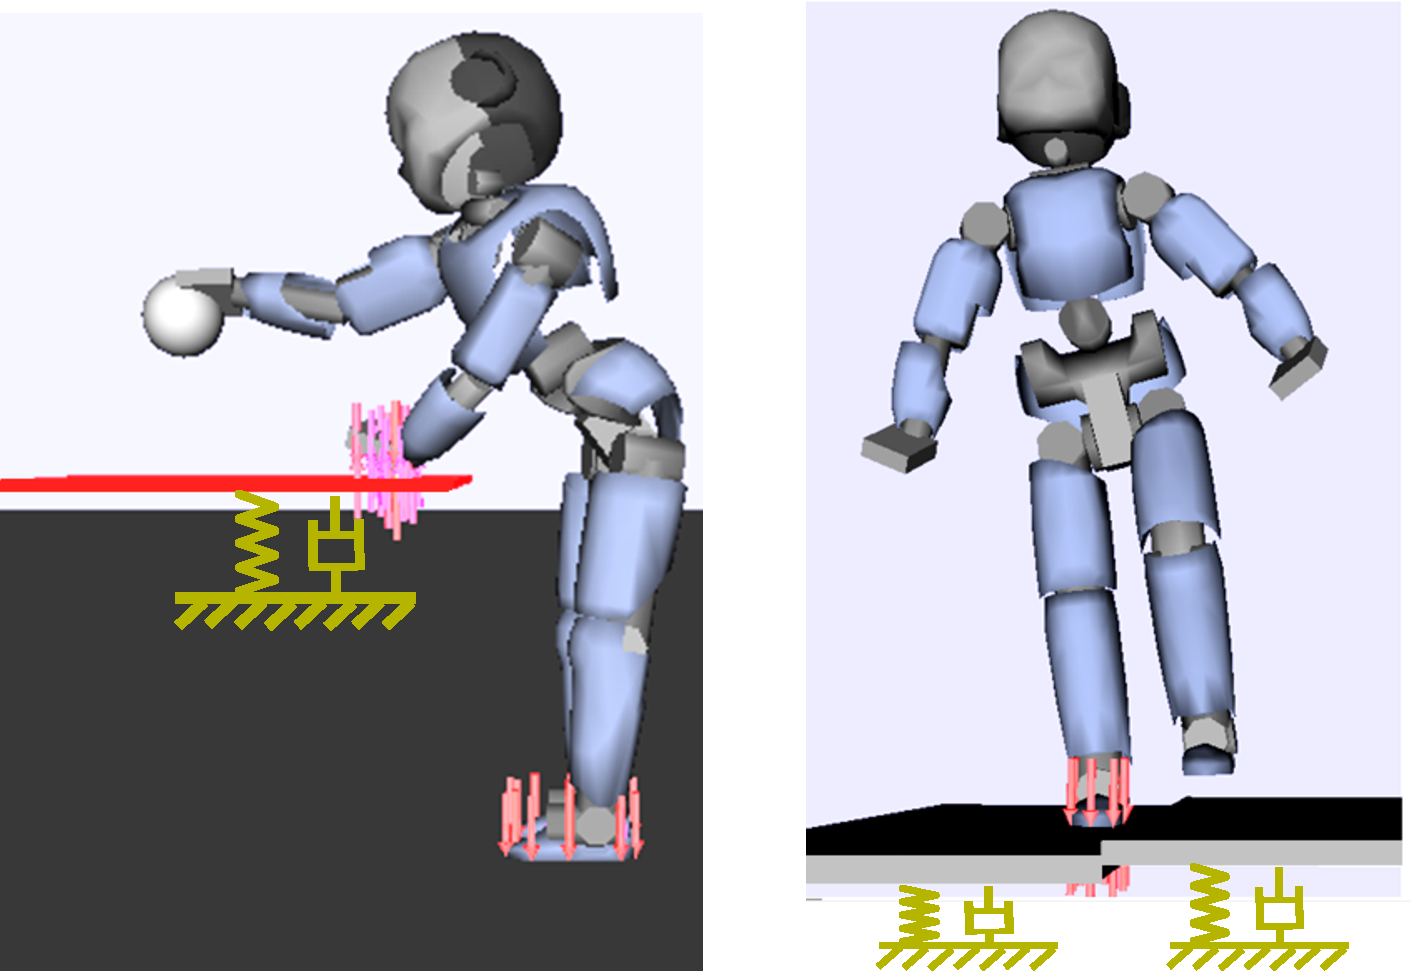
\includegraphics[width=.8\linewidth]{figure/scenario.pdf}
\caption{Examples of balancing on non-rigid contacts during whole-body task execution.}
\label{reaching}
\end{figure}

The contribution of this work consists in a reactive controller for whole-body balancing of humanoid robots performing whole-body tasks in unknown compliant environments. As the motions and forces at support contacts are related to whole-body task executions, their reference trajectories are unavailable a priori. Therefore, this approach focuses on the regulation of contact forces in a reactive way. It reacts to the motions of non-rigid contacts in real-time during whole-body movements, with the aim of establishing contact equilibrium quickly.\\

A frictional non-rigid contact model is proposed both for simulation and for control. The model parameters of the non-rigid environment are unknown to the controller. The force regulation approach does not try to estimate the impedance parameters of the environment, but it regulates contact forces by reacting to environment motions directly. This reactive control approach is embedded in an optimization based multi-task controller of type (1), which has been used to achieve whole-body control of humanoid robots in rigid environments. However, the reactive principle of the approach proposed here is general and can also be applied in many other whole-body controllers to handle non-rigid support contacts. Examples using this approach are provided, where a humanoid robot performs reaching and stepping actions in a non-rigid environment. Further research directions related to this approach are also presented. Details can be found in the paper hereafter included.

\subsection{Reactive whole-body control for humanoid balancing on non-rigid unilateral contacts}
\label{app:liu_IROS2015}
\newpage
\includepdf[pages={1-7}]{appendix/paper_liu-padois_IROS2015.pdf}

\section{Balancing on compliant contacts: model-based control approach}

When a model of the environment is available or has been incrementally learnt, using this model does not only provide the necessary adaptation to the new conditions but allows to obtain efficient behaviours that could not be obtained otherwise. It thus makes much sense to try to model the compliant environment.

\subsection{Model modifications induced by compliant contacts}

When dealing with compliant contacts, modifications are induced in the equation of motion and kinematic constraints expression. The former writes
\begin{equation}
{M}(q) {\dot{\nu}}+{C}({q},{\nu}){\nu} + G(q) = {B} {\tau} + J^\top_{rigid} (q) f_{rigid} + J^\top_{comp} (q) f_{comp}, \label{eq:compliant dyn model}
\end{equation}
while the latter is decomposed in two sub-equations
\begin{subequations}\label{eq:kin constraints}
\begin{eqnarray}
J_{rigid}(q) \dot\nu + \dot{J}_{rigid}(q) \nu & = & 0 \label{eq:kin constraints rigid}\\  
J_{comp}(q) \dot\nu + \dot{J}_{comp}(q) \nu & = & \ddot{p}_{\mathcal{C}_{comp}}\label{eq:kin constraints comp},%(p_{\mathcal{C}_{comp}},R_{\mathcal{C}_{comp}},\dot{p}_{\mathcal{C}_{comp}},\omega_{\mathcal{C}_{comp}},\dot{f}_{comp}) \label{eq:kin constraints rigid},
\end{eqnarray}               
\end{subequations}
where $J^\top_{rigid} (q)$, $f_{rigid}$, $J^\top_{comp} (q)$ and $f_{comp}$ respectively represent the contact Jacobian in the rigid contact directions, the associated rigid contact wrench, the contact Jacobian in the compliant contact directions and the associated compliant contact wrench. Without loss of generality, contacts are here supposed to be either strictly rigid or compliant\footnote{A given contact point can actually be rigid in some direction while compliant in other orthogonal ones.}. $\ddot{p}_{\mathcal{C}_{comp}}$ is the compliant contact points linear and angular acceleration which is assumed to be a function of the state of the contact points and of the derivative of the compliant contact wrench\footnote{As an intuition, consider the example of a mono-dimensional spring-damper system described by the scalar relation $ f = K (x-x_0) + b \dot{x} $, the contact point acceleration can be written $\ddot{x} = \frac{1}{b} ( \dot{f} - K \dot{x})$.} $\ddot{p}_{\mathcal{C}_{comp}} = z\left(p_{\mathcal{C}_{comp}},R_{\mathcal{C}_{comp}},\dot{p}_{\mathcal{C}_{comp}},\omega_{\mathcal{C}_{comp}},f_{comp}\right)$.

 

\subsection{Augmentation of the relative degree of the controlled outputs}

From the modified model, it can be shown that $f$ cannot be considered as an independent intermediate control input any longer as its evolution is subject to the contact points dynamics which is a function of $\dot{f}$. $\dot{f}$ becomes the new independent intermediate control input and it can be concluded that compliant contacts augment the relative degree of the controlled outputs. This means that Equation~(\ref{equ:NE equation}) has to be differentiated in order to relate $\dot{f}$ to the desired center of mass behaviour. The computed contact force derivative can then be fed into Equation~(\ref{eq:kin constraints comp}). Assuming that a good measurement of the compliant contact forces is available and that $z$ can be estimated with high bandwidth and precision through measurement, whole-body dynamics estimation and/or contact model parameters estimation, one can then directly solve the whole-body control problem.\\

Even if not formulated in this way, this is the approach retained in \cite{AzadIROS2015} where a ``practical'' implementation is proposed. The proposed controller regulates both linear momentum and angular momentum about the center of mass of the robot by controlling the contact forces at soft contact surfaces\footnote{rigid contact can be accounted for as well without modifying the proposed method itself and with the advantage of easing the estimation of the state of the floating base}. Assuming that contact forces at the compliant surfaces are known (i.e. via force-torque sensors) at the current instant, desired contact forces at the rigid contacts are calculated in order to provide the required rate of change of the robot's momentum.  However, since compliant contact forces are functions of surface deformations, there is not  any control on them at the current instant. Nonetheless, it is possible to control those forces in the next instant by controlling the acceleration of the contact points.  This can be done by predicting one step ahead in time the compliant contact forces given the currently measured ones and the contact model $z$. To implement the proposed method in practice, stiffness and damping coefficients of the contact model have to be estimated beforehand by using contact model parameter estimation methods such as in \cite{Dallalietal13}, \cite{Diolaitietal05}, \cite{Ericksonetal03}. Details of the proposed implementation can be found in the paper hereafter included.

\newpage
\includepdf[pages={1-6}]{appendix/paper_azad-mistry_ICRA2015.pdf}

\subsection{Making use of reasonable rigidity assumptions}

 However, estimating $z$ with high bandwith and precision is a very complex problem and relying on such an assumption is doomed to fail. 

%Balancing is possible only if rigid contacts are available. Non rigid contacts induce a motion of the contact point and cannot provide the support contact forces needed to compensate for the under-actuation of the floating base. The controller introduced in section~\ref{app:liu_IROS2015} actually aims at reaching rigid contact situations as fast as possible thus reducing the transient period during which the robot is actually ``sinking'' in the ground or contact surface. Then, assuming a contact state has been reached where some rigid contacts are available for support, one still needs to account for the compliant behaviour in some contact directions.  

%\section{Whole-Body control and the CoDyCo contribution}
%
%With the emergence of humanoid robots and virtual humans, a fairly large research effort is concentrated on the control of these systems. They are indeed complex by nature and their control remains an opened research question.\\
%
%First, humanoids are free-floating, underactuated systems, \textit{i.e.} systems whose configuration is described by their $n$ joint angles and their 3D pose expressed in some inertial frame\footnote{This pose in SE(3) can be locally described using a minimal number of 6 coordinates.}, while only the joints are directly actuated. Their control is possible thanks to the existence of contacts with the environment\footnote{These contacts are generally located at the feet but can potentially occur anywhere at the surface of the robot.}. These contacts generate wrenches applied to the robot that provide, if properly used, the missing actuation capabilities of the system. While these contacts are necessary, they are challenging as:
%\begin{itemize}
%\item their existence is conditionned by several conditions: 
%\begin{itemize}
%\item contact points (\textit{e.g.} feet) can push on the environment (\textit{e.g.} ground) but not pull: contacts are unilateral;
%\item the contact forces have to lie in their associated Coulomb friction cone to avoid slippage;
%\item the dynamic wrench applied at the center of mass of the robot has to be controlled in such a way that it can actually be compensated for by the contact forces and thus avoid tipping over.
%\end{itemize}
%\item they largely constrain the pose of the contact points and thus the overall motion of the system;
%\item they are discrete in nature: contrarily to wheeled systems, modifying the location of the contact point in a controlled manner\footnote{i.e. without slipping.} requires to break contact.
%\end{itemize}
%
%The second source of complexity comes from the large number of degrees of freedom (DOF) and the tree structure of these systems. These characteristics imply what is generally called "redundancy" and provide the system with the capability to perform several tasks concurrently. While redundancy is appealing, the execution of different tasks may not always be compatible and proper hierachization has to be performed at the control level in order to ensure that safety-critical tasks are not disturbed by less critical ones. This has a fairly large computational complexity.\\
%
%Finally, the control of such systems requires:
%\begin{itemize}
%\item a fairly good knowledge of their kinematic and dynamic model;
%\item access to measures or estimation of contact point locations (and potentially measures of forces if they are to be precisely controlled);
%\item a measure of their 3D pose/velocity/acceleration in some inertial frame;
%\item a torque controlled robot.
%\end{itemize}
%Modeling and identifying the model parameters is thus of major importance. Proper sensing (joint level odometry, force/torque sensing, inertial measurment units) and estimation capabilities are also mandatory.
%
%\subsection{Whole-body control: global vs local control problem} 
%
%Solving the global whole-body control problem as a whole, \textit{i.e.} finding at each control instant the adequate actuation torque given some high level mission description such as "Move object A from place B to C", is beyond reach. As a consequence, what is meant by whole-body control often corresponds to a local control problem, less complex than the global one.\\
%
%The main assumption is that the operational tasks\footnote{Operational space tasks are often expressed in 3D space and associated to end-effectors but the concept can be extended to any space that can be expressed as a function of joint space coordinates, including the joint space itself.} to perform at time t in order to achieve a global goal are given. For simple missions, these tasks, their associated goals and relative importances are very often predefined in a very \textit{ad hoc} way. This is hardly possible when considering the specific problem of changing the contact points location and controlling balance. Indeed, although the dynamics of multibody systems are well understood, direct approaches to resolve the motion of all degrees of freedom for locomotion is computationally intractable in real-time due to their large number and to the non-linear behaviour of the system.\\
%
%In fact, to generate dynamically balanced locomotion trajectories efficiently, current methods are based on simplified models of the robot dynamics \cite{SpringerHandb}. One of the most widespread model is the Inverted Pendulum Model (\emph{IPM}) \cite{3Dlinearinve}, where the mass of the robot is assumed to be concentrated at its center of mass (\emph{CoM}). Although more accurate models are sometimes required \cite{RMPmodelfor}, the simple IPM is suitable for many situations where the rotational inertial effects of the robot arms, legs and torso are negligible or can compensate for each other. An example of such a scenario includes walking at a moderately fast pace. When all the contacts are coplanar, a point, sometimes called the Zero Moment Point (\emph{ZMP}) \cite{zmpreview}, that is of particular interest can be defined. Although this name has led to confusion about its physical nature \cite{posturalstabi}, it is often used. A system is considered dynamically balanced if the ZMP lies within the support region, i.e. the 2D convex hull of the contact points \cite{stabilitywalk}. In the IPM, the relationship between the CoM and ZMP dynamics is defined by nonlinear differential equations. However, if the vertical displacements of the CoM are set in advance, the relationship can be decoupled and expressed as linear differential equations. This substantially simplifies the problem into one that can be more efficiently and easily implemented for locomotion trajectory generation and gait control. The trajectory generation problem has been studied through analytical approaches \cite{motionpattern,analyticalgai,walkingallowi}, and more recently, using convex optimization with constraints on the ZMP in discrete time \cite{fastequilibra,walkingpatter,LMPCwalkingw,LMPCforwalki,locomotionvia,walkingwithou}. The efficiency of convex optimization solvers allows them to be used within model predictive control (\emph{MPC}) schemes. This is important in the real-time implementation of reactive walking. However, the ZMP+MPC approach suffers from two main drawbacks: 1) the trajectory of the CoM height ($z$-direction) must be known or fixed in advance, and 2) the contact points must always be coplanar, making this approach unsuitable for walking in complex unstructured environments or if the arms are to also be used. Due to these two restrictions, the ZMP+MPC approach can be regarded as a 2D CoM planner that operates in the horizontal $xy$-plane only.\\
%
%If real-time is not a constraint, motion planning techniques based on probabilistic searches \cite{planningalgor} have been extended to humanoids and can also be used, mostly in an offline fashion, to generate feasible motions for the overall system \cite{hauser2008motion,dalibard2013dynamic,bouyarmane2012humanoid,lengagne2013generation}.\\ %In contrast with these works, the recent work of Tassa \textit{et al.} is a step toward plausible on-line whole-body motion optimization \cite{tassa2014control}.\\
%
%Overall, given the assumption that tasks are provided, the local whole-body control problem can be formulated as follows: at each control time, given a set of $n_t$ tasks to be perfomed and their relative importance, find the (locally) optimal joint torques and contact wrenches such that the task errors are minimized while respecting the task hierarchy, the equation of motion and physical constraints acting on the system (joint limits, joint velocity and joint torque limits, obstacle avoidance). The contact locations are supposed to be known and compatible with the overall desired motion of the system in terms of dynamic equilibrium/balance. The problem to be addressed is thus a very general problem of multi-tasks hierarchical control applied to humanoids.
%
%\subsection{Hierarchical control}
%
%Approaches to maintain a desired task hierarchy using a multi-objective controller draw a lot of interest. This section reviews some classical types of hierarchical control frameworks, as well as the methods for priority representation and transitions within these frameworks.
%
%\subsubsection{Approaches for handling a strict hierarchy}
%\label{sec:Approaches for handling a strict hierarchy}
%
%The simultaneous management of multiple objectives is a well known problem in Robotics. The most popular method to deal with a set of tasks is a hierarchical framework \cite{Liegeois1977}: objectives are prioritized and low priority objectives are carried out only if they do not impact the achievement of top priority objectives. This analytical\footnote{"Analytical" means that an inverse is explicitly computed contrarily to "optimization-based" approaches where the computation of the inverse is implicit.} method is based on null-space projections and can ensure that lower priority tasks are executed only in the null-space of higher-priority tasks, by means of the appropriate design of a null-space projector. At the velocity kinematics level, this approach is generalized with the notion of \textit{stack of task} \cite{Mansard2007}. Based on this framework, many kinds of inversion-based control problem resolutions have emerged: potential fields and gradient projection methods \cite{Khatib1986,Maciejewski1985}, weighted inversion techniques \cite{Chan1995,Huo2011}, clamping \cite{Baerlocher2004}, etc. They have also been extended to the dynamics level \cite{Khatib1986,Hsu89,Peters08}. Despite the fact that most constraints are naturally expressed as inequalities (\textit{e.g.} maximum actuation torques), these resolution schemes are    relying on linear algebra and matrix inversions and thus express them as equalities, \textit{i.e.} in way similar to the way tasks are expressed. These constraints-related tasks aim at getting away from the constraint (active avoidance). The number of constraints being potentially higher than the number of DOF, they mostly fail in highly constrained cases and cannot lead to control solutions that can strictly guarantee the respect of all constraints. One way to circumvent this limitation rely on the appropriate activation of the constraints based on their level of criticity at each instant. This allows the reduction of the number of tasks to be achieved at a given instant but leads to potential discontinuities in the generated control solution. To deal with these discontinuities dedicated developments have been led: adaptative gains for weighting techniques \cite{Chaumette2001}, smooth tasks transitions \cite{Padois2007}, progressive clamping \cite{Raunhardt2007} and dedicated inversion operator \cite{Mansard2009a}.\\
%
%These techniques have also been adapted to humanoid systems at the velocity \cite{Mistry07,Mistry08} and torque \cite{Sentis04bis} levels. In the case of humanoids, the motion of the overall system should be compatible with the contact constraints and, the constraint being expressed at the velocity level, active avoidance is not an appropriate solution. Instead, projected inverse dynamics schemes have been developed \cite{Aghili05,Khatib08,Sentis10,Righetti_IJORR_2013,DelPreteThesis2013} in which tasks are projected into the null-space of the Jacobian of contact constraints.\\
%
%Deciding when a constraint should be activated remains a problem in these approaches \cite{Rubrecht2011b} and, as in the seminal work in \cite{Faverjon1987}\footnote{In \cite{Faverjon1987}, an obstacle avoidance technique includes a control law structure based on a Quadratic Programming (QP). This method limits the velocities toward obstacles using inequalities.  Avoidance is thus passive (does not require motion) which is more likely to avoid the collisions whatever the number of obstacles.}, control approaches relying on optimization tools such as Linear Quadratic Problem solver have emerged \cite{Abe07,Collette07}. These solvers are designed to optimally choose the subset of constraints that should be considered when computing the optimal solution of the control problem. The strong mathematical background in convex optimization is such that optimization based methods mostly outperform analytical methods attempting to heuristically activate constraints as in \cite{Flacco12, Flacco12bis}.\\
%
%More recently, to deal with prioritized inequality constraints more easily, hierarchical quadratic programming (HQP) approaches use numerical QP solvers to solve a Hierarchical Quadratic Program \cite{Kanoun09}. 
%%An advantage of these approaches is that they can deal with prioritized inequality constraints \cite{Kanoun09}. 
%The idea of HQP is to first solve a QP to obtain a solution for a higher priority task objective; 
%and then to solve another QP for a lower priority task, without increasing the obtained minimum of the previous task objective. This prioritization process corresponds to solving at best lower-priority tasks in the null-space of higher-priority tasks.
%The HQP algorithm is applied for solving prioritized inverse dynamics \cite{Saab11} and is also applied to whole-body motion control under unilateral constraints \cite{Saab13}.
%It requires to solve as many QPs as priority levels, which can be quite time consuming. The computation cost of hierarchical inverse kinematics with inequality constraints is improved by an algorithm developed in \cite{Escande14}, which permits real time control of the HRP-4 humanoid robot. Similar work is performed in \cite{HerzogIROS2014} where a reduction of the equation of motion allows for real time control of the SARCOS humanoid robot.\\ 
%
%Generally, for an approach based on strict hierarchy, the relative importance of one task with respect to another one of different priority level is parametrized in a binary way: either strictly higher or strictly lower.
%However, in many contexts, organizing tasks by assigning them with strict priorities is not generic, \textit{i.e.} can have some limitations. First, a strict priority is just an extreme case of the relations of task importance levels. In fact, a task may not always have a strict priority over another one and it is usually difficult to define a strict hierarchy among a set of tasks. 
%%It might not be necessary to strictly prevent a lower priority task from interfering with a higher priority task, as long as the performance of the higher priority task is acceptable. 
%Second, strict priorities can sometimes be too conservative so that they may completely block lower-priority tasks. 
%%Unlike a discrete parametrization of task priorities, a continuous parametrization is richer and more informative. Therefore, this work handles task priorities, which can be strict or non-strict, by using a continuous parametrization. Moreover, priorities are defined here by pairs of tasks: this choice extends the classical notion of priority in Robotics while still making it possible to represent standard lexicographic orders as defined in \cite{Saab13}. 
%
%\subsubsection{Weighting strategy}
%Non-strict priorities are usually handled by control approaches using weighting strategies \cite{Abe07,Collette07,Liu11,Salini11,Bouyarmane11}.
%These control frameworks solve all the constraints and task objectives in one QP and provide a trade-off among task objectives with different importance levels. 
%As the performances of higher priority tasks cannot be guaranteed by simply adjusting the weights of task objectives, a prioritized control framework is proposed in \cite{Liu12} to ensure the performance of a higher-priority task within a user defined tolerance margin. However, this approach handles priorities of only two levels. 
%In approaches based on weighting strategies, task priorities can be parametrized continuously. Nonetheless, even though the work in \cite{kerrigan2000} on soft constraints in model predictive control could probably be adapted to provide a way to reach the extreme case of strict priorities, the existing robotic applications of these frameworks do not extend to strict hierarchies.
%
%%The control framework proposed in this paper is based on these frameworks: it formulates and solves all tasks and constraints in one QP. It also largely outperforms them by permitting priorities to change continuously from a non-strict case to a strict case.
%
%\subsubsection{Task transitions}
%Earlier versions of analytical methods and HQP approaches can ensure strict priorities among tasks; however, a change in the task set, such as a swap of task priorities, may lead to discontinuity. Recently, different methods have been developed to handle task transition problems.
%An approach to smooth priority rearrangement between two tasks is proposed in \cite{Keith11,Petric13}. Approaches for continuous and simultaneous transitions of multiple tasks are developed in \cite{Mansard09bis,Lee12}. A specific inverse operator is proposed  in \cite{Mansard09bis} to ensure continuous inverse in the analytical computation of control laws. The approach presented in \cite{Lee12} is based on intermediate desired values in the task space. When the number of task transitions increases, this approach recommends to use an approximation to reduce the computational cost.
%Smooth task transitions can be easily achieved within a framework using a weighting strategy by the continuous variation of task weights \cite{Salini11}.
%
%\subsection{Controllers developped within the framework of CoDyCo}
%
%The whole-body controllers developped and implemented by UPMC and IIT  within the framework of the CoDyCo projects are mostly related to the work of:
%\begin{itemize}
%\item Joseph Salini at UPMC whose PhD thesis addressed the topic of "Dynamic control for the task/posture coordination of humanoids: toward synthesis of complex activities" \cite{Salini12};
%\item Andrea Del Prete at IIT whose PhD thesis addressed the topic of "Control of Contact Forces using Whole-Body Force and Tactile Sensors: Theory and Implementation on the iCub Humanoid Robot" \cite{DelPreteThesis2013};
%\item Mingxing Liu at UPMC whose postdoctoral work has been focused on "Generalized Hierarchical Control" \cite{generalizedsm}\footnote{The submitted version of this article is provided in Appendix~\ref{app:GHC}}.
%\end{itemize}
%
%On one hand, the work of Salini deals with the general problem of dynamic control of “task-oriented” under-actuated and redundant systems considering more specifically the humanoid robotic systems or virtual humans. It brings contributions to the problem of motor activities synthesis for constrained systems by their intrinsic capacities and by particular physical interactions with the environment. More specific issues that are addressed relate to:
%\begin{itemize}
%\item the dynamic control of humanoid systems for carrying out basic activities requiring task/posture coordination perturbed by physical interactions;
%\item the building of sequences of continuous dynamic activities based on a repertoire of motor coordination;
%\item the planning and the adaptation of activities in the aim of a supervised automatic sequencing for complex non-deterministic tasks.
%\end{itemize}
%The major outcome of this work is a generic controller based on the completion of several tasks under constraints. As mentionned in Sec.~\ref{sec:Approaches for handling a strict hierarchy}, these constraints are mainly the representation of physical limitations of the robot, both internal, such as joint limits, and external as frictional contacts during interactions with the environment. The formalism is based on "task functions", the simultaneous resolution of several of them is realized by a quadratic multicriteria optimal control scheme. It is based on convex optimization methods, and the good properties of quadratic programming (QP) can efficiently perform the whole body control (in time, convergence, robustness) for the task/ posture coordination. A strategy based on weights is used to manage conflicting tasks. It allows a great flexibility of control during transitions in the sets of tasks and constraints for the continuity of the control variables. This controller has been implemented in a Arboris-Python, a physics engine also developped by Salini \cite{Arboris-Python}, on a virtual model of the iCub robot. These experiments illustrate the achievement of multi-task problems and exhibit the good  performance of the controller for managing transitions in task sequences or when state change in the set of constraints, when a contact is broken, for example. In addition, program performance optimization of a temporal point of view are studied for different formalisms. On top of this whole-body controller, Salini has also developped a high-level controller to plan and adapt sequences of tasks for the realization of more complex activities based on a predetermined repertoire of actions and monitoring their performance, while ensuring the continuity of the  control variables .\\
%
%On the other hand, the objective of the PhD thesis of Del Prete was to improve the abilities of humanoid robots to interact with their surrounding. In particular, the idea of integrating force and touch feedback was investigated, so as to control the robot in presence of external forces acting on any part of its body. To this aim, this work exploited the humanoid robot iCub as test platform, and it tackled three main issues:
%\begin{itemize}
%\item spatial calibration of tactile sensors;
%\item estimation of contact forces using tactile sensors and force/torque sensors;
%\item prioritized position and force control.
%\end{itemize}
%The major outcome of this work was the synthetis a new framework for strictly prioritized position and force control of floating-base robots. The framework was compared to other state-of-the-art similar frameworks, both analytically and in simulation, and it proved preferable in terms of optimality and computational efficiency — twice as efficient, while preserving the optimality of the solution. Moreover, a method for estimating the 3D positions of tactile sensors was proposed. The method relies on force/torque measurements and it was exploited to calibrate the 1500 tactile sensors mounted on the arms of the iCub robot, with an average error of approximately 7 mm. Another method was introduced, which makes use of the calibrated tactile sensors, together with the distributed force/torque sensors, to estimate an arbitrary number of contact forces acting on any part of the robot’s body. The method is based on the Recursive Newton-Euler Algorithm, and it was implemented as part of  the open-source C++ library iDyn. Furthermore, a theoretical and empirical analysis investigated how incorrect estimation of contact points may affect the resulting contact forces and induce undesired joint accelerations. Tests on the iCub robot demonstrated a significant improvement in the performance of the force controller when the tactile system was used.\\
%
%Finally, with the aim of handling both strict and non-strict hierarchies simultaneously, and achieving smooth transitions of priorities, a novel control framework called Generalized Hierarchical Control (GHC) has been developped at UPMC in the work of Liu. The contributions of this work are as follows:
%\begin{itemize}
%\item the development of a generic dynamic control framework, which solves a single quadratic program (QP) to account for an arbitrary number of strict and non-strict task priorities;
%\item the development of a generalized projector, which ensures desired task priorities, their smooth transitions as well as an elegant way of inserting and deleting tasks among those to be performed. The implementation of such a projector is not restricted to the dynamic control framework. In fact, it can be implemented in many analytical and optimization-based control frameworks. Task priorities can be handled by the modulation of a priority matrix, without the necessity of modifying the control problem formulation each time the priorities change. This projection matrix regulates to what extent a lower-priority task is projected into the null-space of a higher-priority task. In other words, it allows a task to be completely, partially, or not at all projected into the null-space of some other tasks. The priority levels can be changed by the modulation of the generalized projector.
%\end{itemize}
%
%\section{Results}
%
%In this section, whole-body control CoDyCo related results obtained both in simulation and on the iCub robot are summarized. The controllers developped by Salini and Del Prete have been ported to C++ during the first months of the CoDyCo project and are now being integrated to the WBI interface developped to provide a common abstraction layer fo whole-body controllers and described in Deliverable 1.2. The controller of Liu is coded in C++ within the XDE simulation framework (see Deliverable 1.1) and a quasi-static version has been developped as a C++ Orocos component \cite{Bruyninckx2001} for the real-time control of the LWR KUKA robot \cite{liu_ICRA2015}.
%
%\subsection{Year~1 scenario: balancing on multiple rigid contact points}
%
%Year~1 scenario has been validated in simulation using Salini's controller in the XDE simulation framework (see Section 4.7 of Deliverable 5.1). It has also been validated using Liu's controller in simulation using the XDE simulation framework \cite{LiuAutRob2014SI}\footnote{The article related to the work of Liu \textit{et al.}  \cite{LiuAutRob2014SI} is provided in Appendix~\ref{app:LiuAutRob2014SI}}.\\
%
%On the real robot, Del Petre's controller has been used has a basis for the integration of Year 1 Demo (illustrated on Fig.~\ref{fig:year1_demo}). The proposed balanced controller is described in \cite{Nori_FRAI2015,Arslan2014}\footnote{The article related to the work of Nori \textit{et al.} \cite{Nori_FRAI2015} is provided in Appendix~\ref{app:NoriFRAI2015}. The internship report of Talha Ali Arslan \cite{Arslan2014} is provided in Appendix~\ref{app:report Arslan}}. Some extension of this work has led to recent developments illustrated in a recently published video\footnote{\url{https://www.youtube.com/watch?v=VrPBSSQEr3A}}. A view of the obtained performance is provided on Fig.~\ref{fig:cool_balancing}.\\
%
%   \begin{figure}[h!]
%      \centering
%      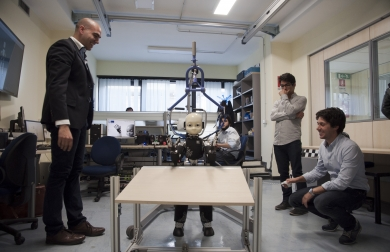
\includegraphics[width=0.45\textwidth]{figure/year1_demo}       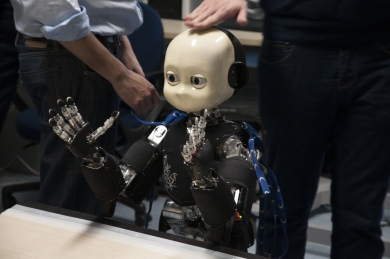
\includegraphics[width=0.45\textwidth]{figure/year1_demo_2}
%      \caption{Views of iCub balancing on multiple contacts using one the whole-body controller developped within the framework of the CoDyCo project.}
%      \label{fig:year1_demo}
%   \end{figure}
%
%    \begin{figure}[h!]
%      \centering
%      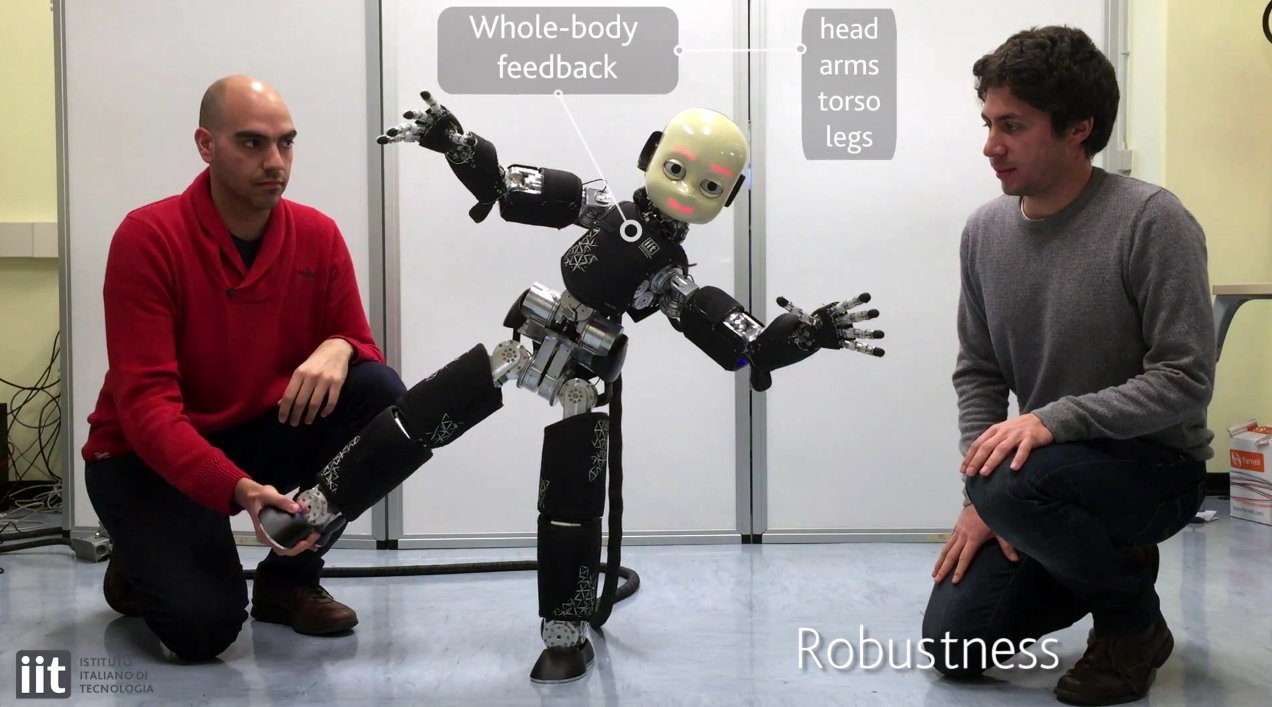
\includegraphics[width=0.8\textwidth]{figure/cool_balancing_demo}
%      \caption{View of the most recent developments in the implementation of the CoDyCo whole-body controller: iCub balancing on one foot while interacting with humans.}
%      \label{fig:cool_balancing}
%   \end{figure}
%
%\subsection{Year~2 scenario: balancing on feet while performing goal directed actions}
%
%Year~2 scenario has been validated in simulation using Salini's controller in the XDE simulation framework in several occasions\footnote{see \url{http://goo.gl/tsT4Iv} for an overview.}. More recently, the work of Lober \textit{et al.} aiming at multiple task optimization using dynamical movement primitives for whole-body reactive control builds on Salini's controller \cite{lober-HUMANOIDS2014}. Fig.~\ref{fig:lober-hum14} and a video\footnote{\url{http://goo.gl/QoSfp7}} accompanying the published work illustrate these results.\\
%
%    \begin{figure}[h!]
%      \centering
%      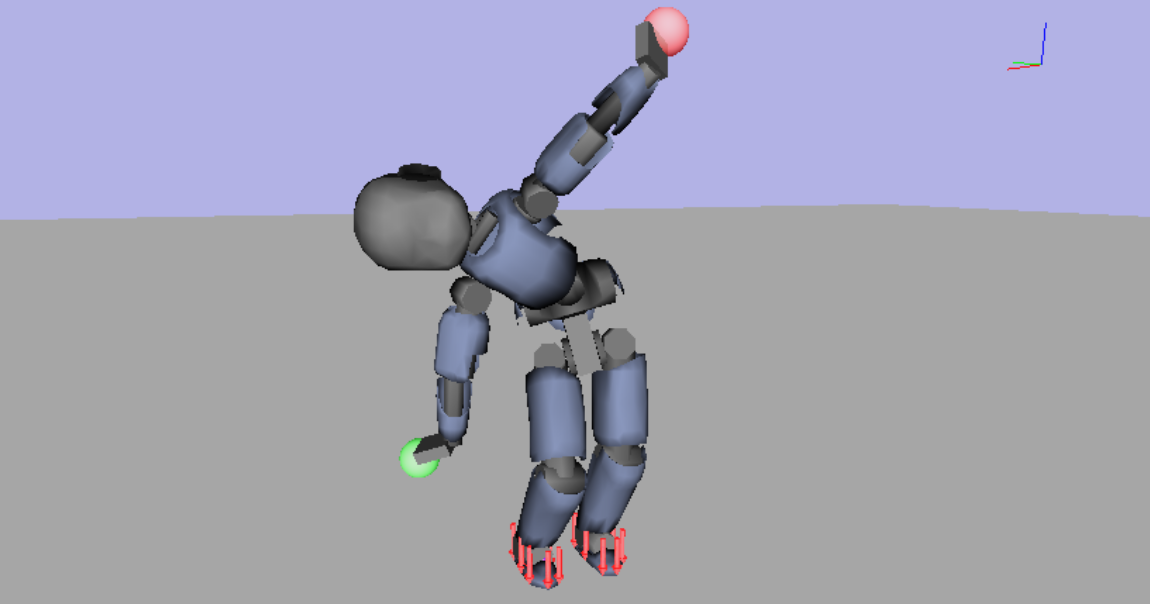
\includegraphics[width=0.8\textwidth]{figure/lober_hum14}
%      \caption{View of some recent developments in the implementation of the CoDyCo whole-body controller in goal oriented actions}
%      \label{fig:lober-hum14}
%   \end{figure}
%
%Fig.\ref{fig:babic_lober_snapshots} provides a view of some recent work performed in coordination with Jan Babic from JSI during his period as a visiting professor at UPMC (November 2014). The goal of this on-going cooperation is to reproduce, using a synthetic whole-body controller, results obtained in human reaching with additional contact experiments in Work Package 2.\\
%
%    \begin{figure}[h!]
%      \centering
%      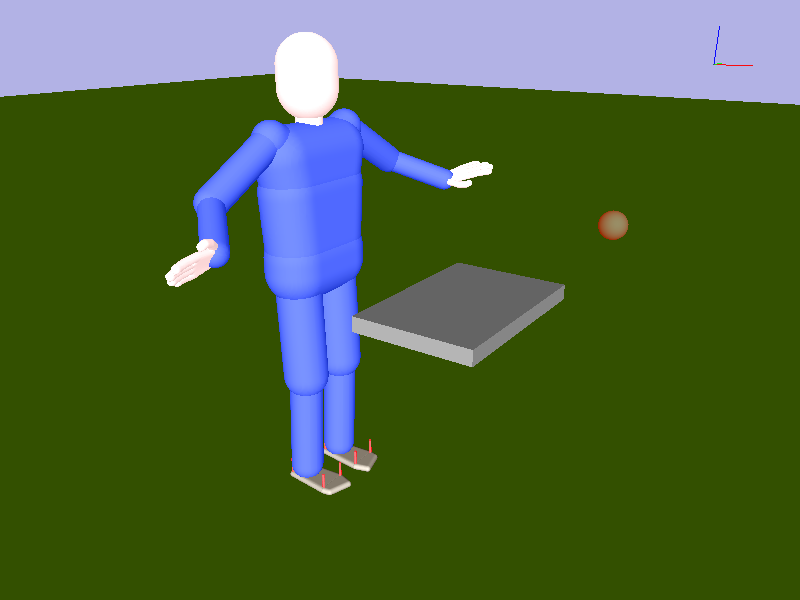
\includegraphics[width=0.24\textwidth]{figure/lober_babic_seq1}
%	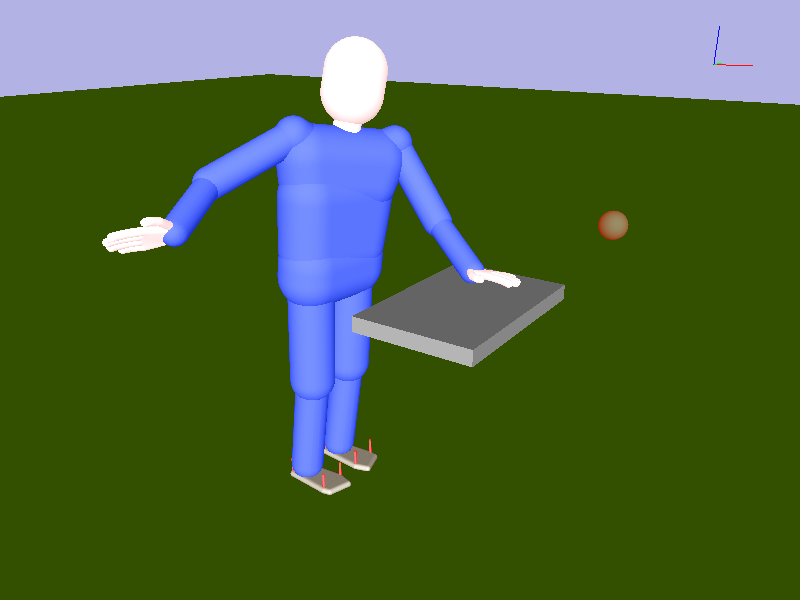
\includegraphics[width=0.24\textwidth]{figure/lober_babic_seq2}
%	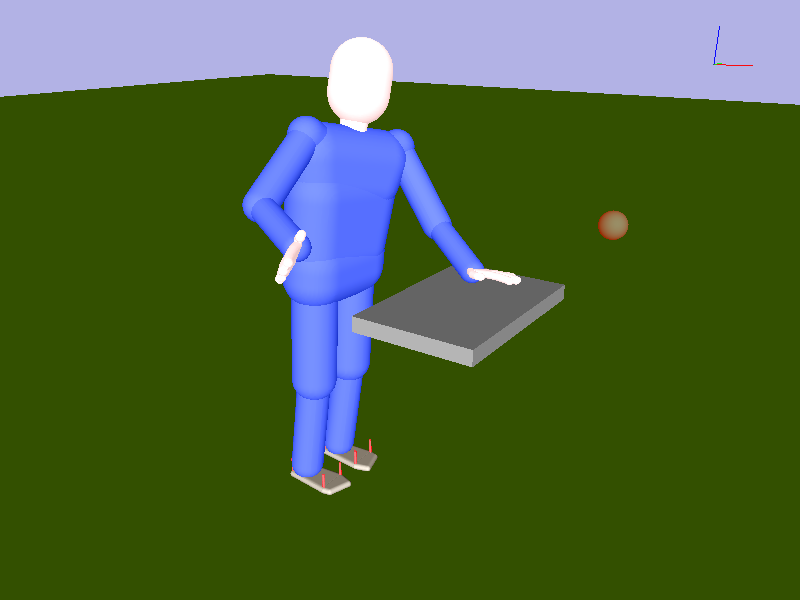
\includegraphics[width=0.24\textwidth]{figure/lober_babic_seq3}
%	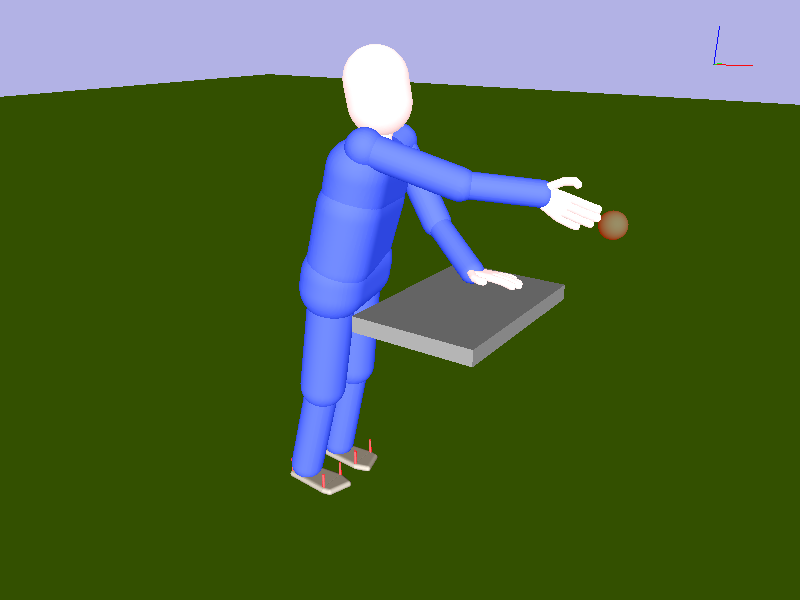
\includegraphics[width=0.24\textwidth]{figure/lober_babic_seq4}
%      \caption{View of a sequence of motion generated using a robotic controller as an attempt to reproduce results obtained in human reaching with additional contact experiments.}
%      \label{fig:babic_lober_snapshots}
%   \end{figure}
%
%
%Year~2 scenario is being currently implemented on the real robot. A description of the scenario and associated controller is provided in Deliverable~5.2.
%
%\subsection{Other use case of interest}
%
%In the work of Ibanez \textit{et al.} \cite{ibanez-IROS2014} a strategy to automatically combined balance strategies based on continuous postural adjustments and discrete changes in contacts is developped in order to maintain postural stability while considering the engaged walking activity. In order to compute optimal time, duration and position of footsteps along with the center of mass trajectory of a humanoid, a novel mixed-integer model of the system is presented. The introduction of this model in a predictive control problem brings the definition of a Mixed-Integer Quadratic Program, subject to linear constraints. Simulation results demonstrate the simultaneous adaptation of the gait pattern and posture of the humanoid, in a walking activity under large disturbances, to efficiently compromise between task performance and balance. In addition, a push recovery scenario displays how, using a single balance-performance ratio, distinct behaviors of the humanoid can be specified. Fig.~\ref{fig:ibanez_iros14} and a video\footnote{\url{http://goo.gl/PjcTcS}} accompanying the published work illustrate the results. As in \cite{ibanez-ICRA2014}, this work builds on the local whole-body controller of Salini and provides the global MPC level needed to generate feasible tasks for the robot.
%
%    \begin{figure}[h!]
%      \centering
%      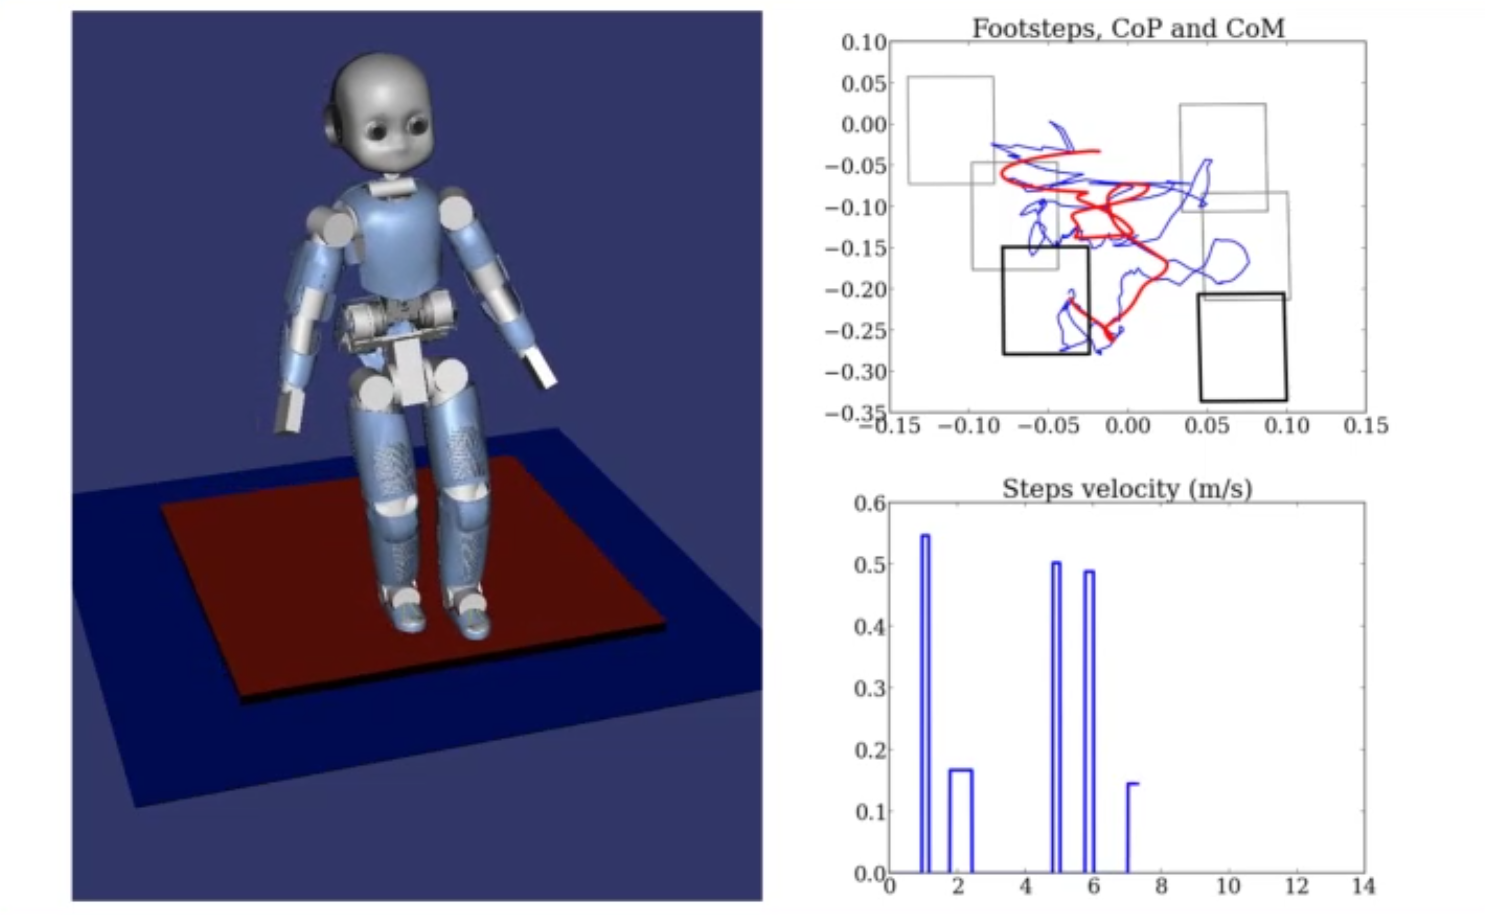
\includegraphics[width=0.8\textwidth]{figure/ibanez_iros14}
%      \caption{A view of iCub automatically adapting its contact locations based on some perceived balance perturbation.}
%      \label{fig:ibanez_iros14}
%   \end{figure}
%
%\newpage{}
%\section{Conclusion}
%
%The CoDyCo consortium has a strong expertise in the domain of whole-body control and is well equipped with state-of-the art whole-body controllers. These controllers are the topic of several research results obtained by the consortium and cited in the results Section of this deliverable. Through the WBI software abstraction presented in Deliverable~1.2, they provide appropriate tools based on which the results of all worpackages can be ported to the iCub humanoid robot. This is already the case for the Year~1 and Year~2 demonstration. 
%




\newpage{}

\phantomsection
\bibliographystyle{IEEEtran}
% argument is your BibTeX string definitions and bibliography database(s)
\bibliography{IEEEabrv,D3.2}
\addcontentsline{toc}{section}{References}

\newpage{}
\begin{appendices}
\appendices

%\section{Generalized Hierarchical Control}
%\label{app:GHC}
%\newpage
%\includepdf[pages={2-16}]{appendix/GHC_Submitted_ISIR_2014.pdf}
%
%\section{Whole-Body Hierarchical Motion and Force Control for Humanoid Robots}
%\label{app:LiuAutRob2014SI}
%\newpage
%\includepdf[pages={1-9}]{appendix/GHCiCub_AutRobSubmitted_ISIR_2014.pdf}
%
%\section{iCub Whole-body Control through Force Regulation on Rigid Non coplanar Contacts}
%\label{app:NoriFRAI2015}
%\newpage
%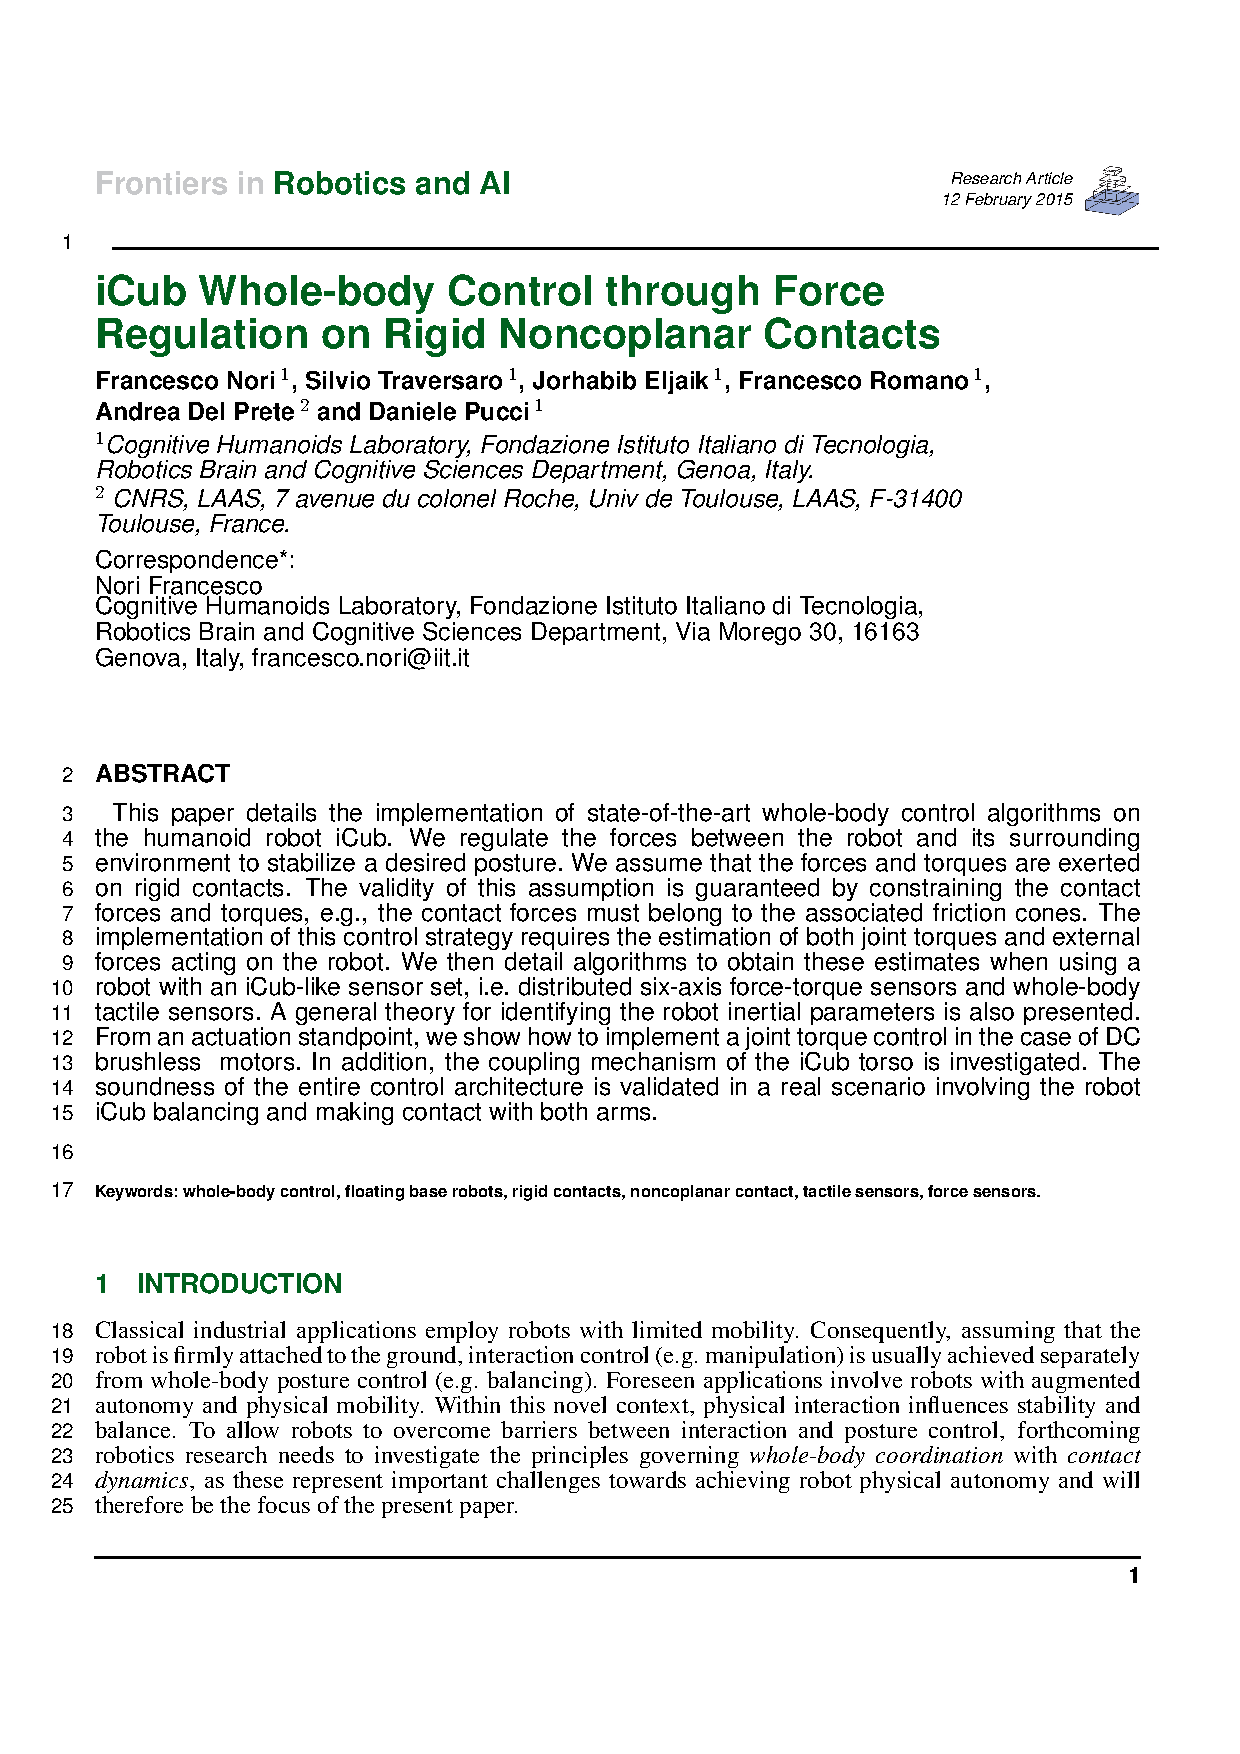
\includepdf[pages={1-27}]{appendix/wholeBodyControl_Frontiers_in_Robotics_and_AI_IIT_2014.pdf}
%
%\section{Improvement of a Balancing Force and Posture Controller with Torque Minimization}
%\label{app:report Arslan}
%\newpage
%\includepdf[pages={1-47}]{appendix/BalanceControl_MastersThesis_Internship_Talha_Ali_Arslan_IIT-TUEindhoven_2014.pdf}

\end{appendices}




\end{document}

%%% Local Variables:
%%% mode: latex
%%% TeX-master: t
%%% save-place: t
%%% End:
